% basics.tex
% Graphs in Computer Science (in Russian)
% Author: Evgeny Simonenko <easimonenko@mail.ru>
% License: CC BY-ND 4.0

\chapter{Основные понятия теории графов}

\section{Основные понятия}

\emph{Графом}\index{Граф} $G$ называют пару конечных множеств $G=(V, E)$ , где 
элементы множества $V$ называются \emph{вершинами}\index{Вершина}, а элементы 
множества $E$ представляют собой пары элементов из множества $V$ и называются 
\emph{рёбрами}\index{Ребро}. Если рёбра в графе представляют собой 
неупорядоченные пары $\{u, v\}$ , то соответствующий граф называют 
\emph{неориентированным}. Если рёбра – упорядоченные пары $(u, v)$, то граф 
называют \emph{ориентированным} (орграфом). В случае орграфов рёбра также 
называют \emph{дугами}. Говорят также, что вершины $u$ и $v$ \emph{соединены} 
ребром.

\emph{Петлёй} называют ребро соединяющее одну и ту же вершину. Граф, у которого 
есть пара вершин, соединённых двумя или более рёбрами, называют 
\emph{мультиграфом}. Граф на рисунке \ref{the koenigsberg bridges} является 
мультиграфом. Граф, не имеющий петель и не являющийся мультиграфом,
называют \emph{простым}.

\tikzstyle{edgelabel} = [font=\footnotesize]
\tikzstyle{graphlabel} = [circle,fill=gray!20]
\tikzstyle{vertex} = [circle,fill=blue!20]

\begin{figure}[h]
	\center
	\begin{tikzpicture}
	\node[vertex] (n1) at (0,2) {A};
	\node[vertex] (n2) at (0,0) {B};
	\node[vertex] (n3) at (0,4) {C};
	\node[vertex] (n4) at (4,2) {D};
	\draw (n1) .. controls (-0.25,1) .. (n2);
	\draw (n1) .. controls (0.25,1) .. (n2);
	\draw (n1) .. controls (-0.25,3) .. (n3);
	\draw (n1) .. controls (0.25,3) .. (n3);
	\draw (n1) -- (n4);
	\draw (n2) -- (n4);
	\draw (n3) -- (n4);
	\end{tikzpicture}
	\caption{Граф задачи о Кёнигсбергских мостах}
	\label{the koenigsberg bridges}
\end{figure}

\begin{equation}
G = (\{A,B,C,D\}, \{\{A,B\}^2,\{A,C\}^2,\{A,D\},\{B,D\},\{C,D\}\})
\end{equation}

Заметим, что мы не накладываем ограничение на мощность множеств $V$ и $E$. Если
$V$ и $E$ являются конечными множествами, то говорят, что граф \emph{конечный}, 
и это обычная ситуация, так что, если не уточняется, то подразумевается, что 
граф конечный. В случае конечного $V$, но бесконечного $E$, мы имеем граф с
бесконечным числом кратных рёбер или петель. В случае с бесконечным $V$, но 
конечным $E$, имеем граф с бесконечным числом изолированных вершин. Наконец, 
если и $V$, и $E$ бесконечны, то такой граф называют \emph{бесконечным}.

Для дальнейшего удобства будем полагать, что $|V|=n$ и $|E|=m$ для случая, когда
множество $V$ или $E$ конечно.

Граф называется \emph{помеченным}, если его вершинам приписаны различные метки. 
Обычно в качестве меток используются натуральные числа в диапазоне от $1$ до 
$n$, где $n=|V|$, часто также применяются строчные латинские буквы. При 
необходимости рёбра также могут быть помечены.

Вершины, соединённые ребром, называются \emph{смежными}. Рёбра, имеющие общую 
вершину, также называются \emph{смежными}. Ребро и любая из его двух вершин 
называются \emph{инцидентными}. Говорят также, что ребро \emph{инцидентно} 
своим вершинам.

Каждый граф можно представить на плоскости в виде множества точек, 
соответствующих вершинами, которые соединены линиями, соответствующими рёбрам. 
В трёхмерном пространстве любой граф можно представить таким образом, что 
линии, соответствующие рёбрам, не будут пересекаться.

Граф, у которого множество $E=\emptyset$, то есть, в котором отсутствуют рёбра, 
называется \emph{нуль-графом}.

Граф называется \emph{полным}, если любые две его вершины смежны. Будем 
обозначать полный граф с $n$ вершинами символом $K_n$.

\begin{figure}[h]
	\center
	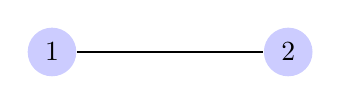
\begin{tikzpicture}[every node/.style={circle,fill=blue!20}]
	\node (n1) at (0,2) {1};
	\node (n2) at (3,2) {2};
	\foreach \from/\to in {n1/n2}
	\draw (\from) -- (\to);
	\end{tikzpicture}
	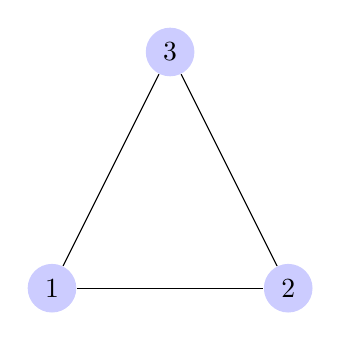
\begin{tikzpicture}[every node/.style={circle,fill=blue!20}]
	\node (n1) at (0,0) {1};
	\node (n2) at (3,0) {2};
	\node (n3) at (1.5,3) {3};
	\foreach \from/\to in {n1/n2,n1/n3,n2/n3}
	\draw (\from) -- (\to);
	\end{tikzpicture}
	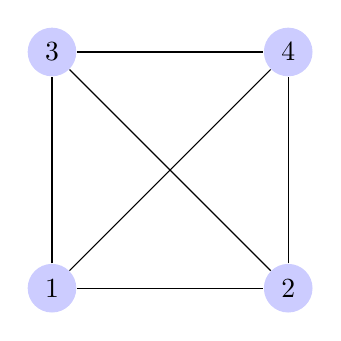
\begin{tikzpicture}[every node/.style={circle,fill=blue!20}]
	\node (n1) at (0,0) {1};
	\node (n2) at (3,0) {2};
	\node (n3) at (0,3) {3};
	\node (n4) at (3,3) {4};
	\foreach \from/\to in {n1/n2,n1/n3,n1/n4,n2/n3,n2/n4,n3/n4}
	\draw (\from) -- (\to);
	\end{tikzpicture}
	\caption{Примеры полных графов: $K_2$, $K_3$, $K_4$}
\end{figure}

Число рёбер в полном графе равно $C^2_n=\frac{n\cdot(n-1)}{2}$. Количество 
помеченных графов с фиксированным множеством вершин $V$, $|V|=n$, равно 
количеству подмножеств множества рёбер полного графа, то есть $2^{C^2_n}$.

Граф $H$ называется \emph{подграфом} графа $G$, если все его вершины и рёбра 
принадлежат графу $G$. \emph{Остовный} подграф – это подграф графа $G$, 
содержащий все его вершины. \emph{Клика} графа – это его максимальный полный 
подграф.

\begin{figure}[h]
	\center
	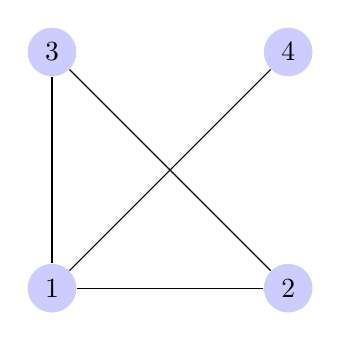
\begin{tikzpicture}[every node/.style={circle,fill=blue!20}]
	\node (n1) at (0,0) {1};
	\node (n2) at (3,0) {2};
	\node (n3) at (0,3) {3};
	\node (n4) at (3,3) {4};
	\foreach \from/\to in {n1/n2,n1/n3,n1/n4,n2/n3}
	\draw (\from) -- (\to);
	\end{tikzpicture}
	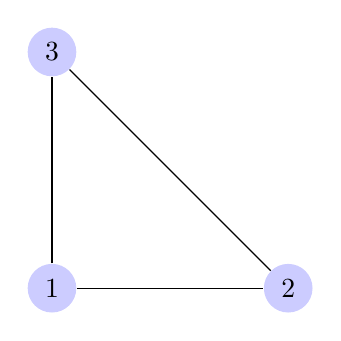
\begin{tikzpicture}[every node/.style={circle,fill=blue!20}]
	\node (n1) at (0,0) {1};
	\node (n2) at (3,0) {2};
	\node (n3) at (0,3) {3};
	\foreach \from/\to in {n1/n2,n1/n3,n2/n3}
	\draw (\from) -- (\to);
	\end{tikzpicture}
	\caption{Пример клики графа}
\end{figure}

Два графа $G$ и $H$ \emph{изоморфны} $(G\simeq H)$, если между множествами их 
вершин можно установить взаимно однозначное соответствие, при котором 
сохраняется отношение смежности. Это означает, что в различных представлениях
эти графы могут выглядеть разными, но структура у них будет одинаковой.

\begin{figure}[h]
	\center
	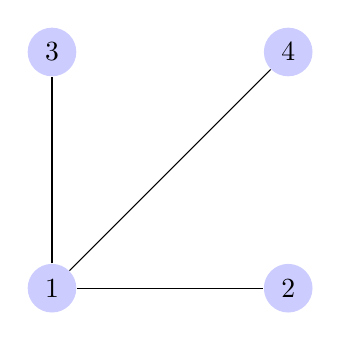
\begin{tikzpicture}[every node/.style={circle,fill=blue!20}]
	\node (n1) at (0,0) {1};
	\node (n2) at (3,0) {2};
	\node (n3) at (0,3) {3};
	\node (n4) at (3,3) {4};
	\foreach \from/\to in {n1/n2,n1/n3,n1/n4}
	\draw (\from) -- (\to);
	\end{tikzpicture}
	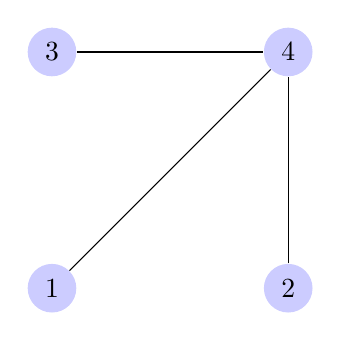
\begin{tikzpicture}[every node/.style={circle,fill=blue!20}]
	\node (n1) at (0,0) {1};
	\node (n2) at (3,0) {2};
	\node (n3) at (0,3) {3};
	\node (n4) at (3,3) {4};
	\foreach \from/\to in {n1/n4,n2/n4,n3/n4}
	\draw (\from) -- (\to);
	\end{tikzpicture}
	\caption{Пример изоморфных графов}
\end{figure}

\emph{Дополнением} $\tilde{G}$ графа $G=(V,E)$ называется граф со множеством 
вершин $V$, две вершины которого смежны тогда и только тогда, когда они не 
смежны в $G$.

\begin{figure}[h]
	\center
	\begin{tikzpicture}
	\node[vertex] (n1) at (0,0) {1};
	\node[vertex] (n2) at (3,0) {2};
	\node[vertex] (n3) at (0,3) {3};
	\node[vertex] (n4) at (3,3) {4};
	\foreach \from/\to in {n1/n2,n1/n3,n1/n4}
	\draw (\from) -- (\to);
	\node[graphlabel] at (1,2) {$G$};
	\end{tikzpicture}
	\begin{tikzpicture}
	\node[vertex] (n1) at (0,0) {1};
	\node[vertex] (n2) at (3,0) {2};
	\node[vertex] (n3) at (0,3) {3};
	\node[vertex] (n4) at (3,3) {4};
	\foreach \from/\to in {n2/n3,n2/n4,n3/n4}
	\draw (\from) -- (\to);
	\node[graphlabel] at (2,2) {$\tilde{G}$};
	\end{tikzpicture}
	\caption{Пример графа и его дополнения}
	\label{complementary graph}
\end{figure}

\emph{Степенью вершины} графа $G$ называется число инцидентных ей рёбер. 
Максимальная степень вершин графа $G$ обозначается $\Delta(G)$, а минимальная – 
$\delta(G)$. Вершина степени $0$ называется \emph{изолированной}, степени 1 – 
\emph{концевой} или \emph{висячей}. Ребро, инцидентное концевой вершине,
также называют \emph{концевым} или \emph{висячим}. На рисунке 
\ref{complementary graph} вершина $1$ графа $\tilde{G}$ изолированная, а 
вершина $4$ графа $G$ – висячая.

Граф $G$, у которого $\Delta(G)=\delta(G)$ называют \emph{регулярным} или 
\emph{однородным}. Очевидно, что любой полный граф является регулярным, также и
нуль-граф.

\begin{figure}[h]
	\center
	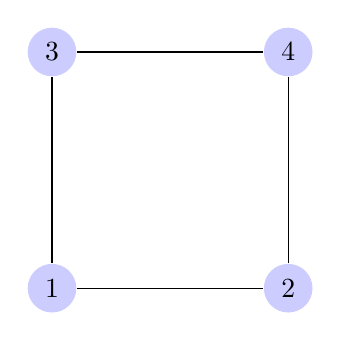
\begin{tikzpicture}[every node/.style={circle,fill=blue!20}]
	\node (n1) at (0,0) {1};
	\node (n2) at (3,0) {2};
	\node (n3) at (0,3) {3};
	\node (n4) at (3,3) {4};
	\foreach \from/\to in {n1/n2,n1/n3,n2/n4,n3/n4}
	\draw (\from) -- (\to);
	\end{tikzpicture}
	\caption{Пример регулярного графа}
\end{figure}

\begin{theorem}[Лемма о рукопожатиях]
	Сумма степеней всех вершин графа равна удвоенному числу рёбер.
	\begin{proof}
		Каждое ребро увеличивает степень одновременно двух вершин. Таким 
		образом, если начать с нулевого количества рёбер, при котором степени 
		всех вершин будут равны $0$, то каждое из <<добавляемых>> рёбер будет 
		увеличивать сумму степеней вершин на $2$.
	\end{proof}
\end{theorem}

Граф называется \emph{транзитивным}, если всегда из того, что вершины $u$ и 
$v$, $v$ и $w$ соединены ребром, при этом $u$, $v$ и $w$ различны, следует, что 
также и вершины $u$ и $w$ соединены ребром. Транзитивный граф, получающийся из 
исходного путём добавления недостающих рёбер, называется \emph{транзитивным 
замыканием}.

\begin{figure}[h]
	\center
	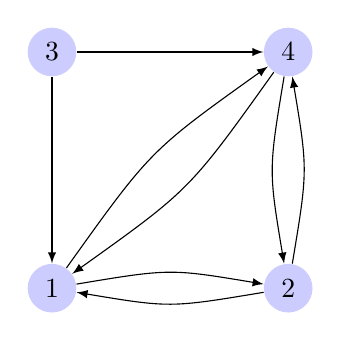
\begin{tikzpicture}[every node/.style={circle,fill=blue!20}]
	\node (n1) at (0,0) {1};
	\node (n2) at (3,0) {2};
	\node (n3) at (0,3) {3};
	\node (n4) at (3,3) {4};
	\foreach \from/\to in {n3/n1,n3/n4}
	\draw[->,>=latex] (\from) -- (\to);
	\draw[->,>=latex] (n1) .. controls (1.25,1.75) .. (n4);
	\draw[->,>=latex] (n4) .. controls (1.75,1.25) .. (n1);
	\draw[->,>=latex] (n1) .. controls (1.5,0.25) .. (n2);
	\draw[->,>=latex] (n2) .. controls (1.5,-0.25) .. (n1);
	\draw[->,>=latex] (n4) .. controls (2.75,1.5) .. (n2);
	\draw[->,>=latex] (n2) .. controls (3.25,1.5) .. (n4);
	\end{tikzpicture}
	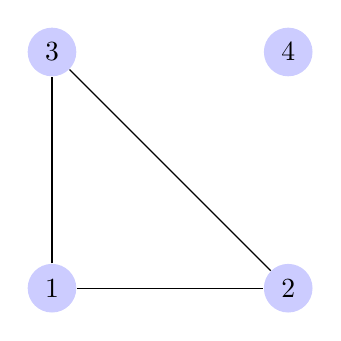
\begin{tikzpicture}[every node/.style={circle,fill=blue!20}]
	\node (n1) at (0,0) {1};
	\node (n2) at (3,0) {2};
	\node (n3) at (0,3) {3};
	\node (n4) at (3,3) {4};
	\foreach \from/\to in {n1/n2,n1/n3,n2/n3}
	\draw (\from) -- (\to);
	\end{tikzpicture}
	\caption{Примеры транзитивных графов}
\end{figure}

\subsection{Упражнения}

\begin{enumerate}
	\item Докажите формулу $C^2_n=\frac{n\cdot(n-1)}{2}$ для количества рёбер графа $K_n$.
	
	\item Докажите формулу $2^{C^2_n}$ для количества помеченных графов с $n$ вершинами.
	
	\item Охарактеризуйте графы, заданные графически (рис. \ref{graphs for exercises}):
	\begin{figure}[h]
		\center
		\begin{tikzpicture}
		\node[vertex] (n1) at (0,0) {a};
		\node[vertex] (n2) at (2,0) {b};
		\node[vertex] (n3) at (4,0) {c};
		\node[vertex] (n4) at (0,2) {d};
		\node[vertex] (n5) at (2,2) {e};
		\node[vertex] (n6) at (4,2) {f};
		\draw (n1) -- (n2);
		\draw (n2) -- (n3);
		\draw (n4) -- (n5);
		\draw (n5) -- (n6);
		\draw (n1) -- (n4);
		\draw (n2) -- (n5);
		\draw (n3) -- (n6);
		\draw (n1) -- (n5);
		\draw (n2) -- (n6);
		\draw (n2) -- (n4);
		\draw (n3) -- (n5);
		\node[graphlabel] at (2,-1) {$G_1$};
		\end{tikzpicture}
		\begin{tikzpicture}
		\node[vertex] (n1) at (0,0) {a};
		\node[vertex] (n2) at (2,0) {b};
		\node[vertex] (n3) at (4,0) {c};
		\node[vertex] (n4) at (0,2) {d};
		\node[vertex] (n5) at (2,2) {e};
		\node[vertex] (n6) at (4,2) {f};
		\draw (n1) -- (n2);
		\draw (n2) -- (n3);
		\draw (n4) -- (n5);
		\draw (n5) -- (n6);
		\draw (n1) -- (n4);
		\draw (n3) -- (n6);
		\node[graphlabel] at (2,-1) {$G_2$};
		\end{tikzpicture}
		\begin{tikzpicture}
		\node[vertex] (n1) at (0,0) {a};
		\node[vertex] (n2) at (2,0) {b};
		\node[vertex] (n3) at (4,0) {c};
		\node[vertex] (n4) at (0,2) {d};
		\node[vertex] (n5) at (2,2) {e};
		\node[vertex] (n6) at (4,2) {f};
		\draw (n4) -- (n5);
		\draw (n5) -- (n6);
		\draw (n1) -- (n4);
		\draw (n2) -- (n5);
		\draw (n3) -- (n6);
		
		\node[graphlabel] at (2,-1) {$G_3$};
		\end{tikzpicture}
		\caption{Графы $G_1$, $G_2$, $G_3$}
		\label{graphs for exercises}
	\end{figure}

	\item Найдите клики в представленных выше графах.
	
	\item Найдите максимальные клики в графе $G_1$.
	
	\item Изобразите граф $K_6$.
	
	\item Найдите дополнения до полного графа для представленных выше графов.
\end{enumerate}

\section{Граф как бинарное отношение}

\emph{Бинарным отношением} $R$ между множествами $X$ и $Y$ называется 
подмножество произведения $X \times Y$, $R \subseteq X \times Y$, и обозначается $X R\,Y$. Если $X = Y$, то бинарное отношение называется \emph{отношением на множестве} $X$, $R \subseteq X^2$. Если $x$ находится в отношении с $y$, то пишут $x R y$. Примерами отношений являются: отношение равенства, неравенство, эквивалентность, отношение порядка.

Очевидно, что с точки зрения теории множеств граф является бинарным отношением.

Множество $X$ бинарного отношения $R \subseteq X \times Y$ называется \emph{областью определения отношения} $R$ и обозначается $\mathrm{Dom} R$. Множество $Y$, соответственно, называется \emph{областью значения отношения} $R$ и обозначается $\mathrm{Im} R$.

Множество обратных пар отношения $R$, $\{(y,x) \mid (x,y) \in R\}$, называется \emph{обратным} или \emph{инверсией} и обозначается $R^{-1}$.

\emph{Композиция} (или \emph{суперпозиция}) бинарных отношений $R$ и $S$ это множество $\{(x,z) \mid \exists y ({x R y} \land {y S z})\}$. Композиция обозначается $R \circ S$.

Бинарное отношение $R$ называется:

\begin{itemize}
	\item[--] \emph{рефлексивным}, если $\forall x \in X \colon (x,x) \in R$;
	\item[--] \emph{антирефлексивным} или {иррефлексивным}, если $\forall x \in X \colon (x,x) \notin R$;
	\item[--] \emph{корефлексивным}, если $\forall {x,y} \in X \colon {x R y} \Rightarrow x = y$;
	\item[--] \emph{симметричным}, если $\forall x,y \in X, x \neq y \colon 
	(x,y) \in R \Rightarrow (y,x) \in R$;
	\item[--] \emph{антисимметричным}, если $\forall x,y \in X \colon (x,y) 
	\in R,(y,x) \in R \Rightarrow x = y$;
	\item[--] \emph{асимметричным}, если $\forall {x,y} \in X: (x,y) \in R \Rightarrow \lnot {(y,x) \in R}$;
	\item[--] \emph{транзитивным}, если $\forall x,y,z \in X \colon (x,y) \in 
	R, (y,z) \in R \Rightarrow (x,z) \in R$;
	\item[--] \emph{евклидовым}, если $\forall {x,y,z} \in X: (x,y) \in R \land (x,z) \in R \Rightarrow (y,z) \in R$;
	\item[--] \emph{полным (или универсальным)}, если $\forall x,y \in X, x 
	\neq y \colon (x,y) \in R \vee (y,x) \in R$;
	\item[--] \emph{нулевым}, если $\forall x,y \in X \colon (x,y) \neq R$.
	\item[--] \emph{коннексным}, если $\forall {x,y} \in X: (x,y) \in R \lor (y,x) \in R \lor x = y$;
	\item[--] \emph{имеющим трихотомию}, если $\forall {x,y} \in X: (x,y) \in R \oplus (y,x) \in R \oplus x = y$.
\end{itemize}

Бинарное отношение может быть задано с помощью \emph{матрицы бинарного отношения}, в которой $1$ обозначает наличие пары $(x,y)$ в бинарном отношении, и $0$ – её отсутствие. В теории графов такую матрицу называют \emph{матрицей смежности}. В случае мультиграфов вместо нулей и единиц указывают количество рёбер между соответствующими вершинами.

Рефлексивность с точки зрения графов означает, что у каждой вершины графа есть
петля. Антирефлексивность, напротив, запрещает петли; простой граф этому 
удовлетворяет. Симметричности удовлетворяют неориентированные графы, и 
ориентированные графы, если каждой дуге соответствует противоположно 
направленная ей. Антисимметричность, напротив, это запрещает. Таким образом,
ни один неориентированный простой граф антисимметричностью не обладает, однако,
граф, у которого есть только петли, уже удовлетворяет. Ориентированные графы, у
которых для любой дуги нет противоположно направленной, также удовлетворяют.
Транзитивному отношению соответствуют так называемые транзитивные графы. Их мы
рассмотрим ниже. Полному графу соответствует универсальное отношение. 
Нуль-графу соответствует нулевое отношение.

Можно заметить, что матрицы смежности графов будут обладать следующими 
свойствами:

\begin{itemize}
	\item[--] при наличии петель на главной диагонали будут попадаться числа, 
	отличные от нуля;
	\item[--] у простого графа на главной диагонали всегда находятся нули;
	\item[--] матрица неориентированного простого графа симметрична относительно
	главной диагонали; симметричность для ориентированного графа означает
	присутствие дуг обоих направлений;
	\item[--] у полного графа все элементы матрицы смежности, кроме, возможно,
	диагональных, ненулевые;
	\item[--] у нуль-графа матрица нулевая.
\end{itemize}

\section{Представление графов}

Здесь мы рассмотрим следующие классические способы представления графов:
\begin{itemize}
	\item[--] матрица смежности;
	\item[--] матрица инцидентности;
	\item[--] список связности;
	\item[--] список рёбер.
\end{itemize}

Указанные способы рассмотрим на примере помеченного простого графа, 
представленного на рисунке \ref{example of a graph}.

\begin{figure}[h]
	\center
	\begin{tikzpicture}
	\node[vertex] (n1) at (2,4) {1};
	\node[vertex] (n2) at (0,2) {2};
	\node[vertex] (n3) at (0,0) {3};
	\node[vertex] (n4) at (4,4) {4};
	\node[vertex] (n5) at (2,2) {5};
	\node[vertex] (n6) at (4,0) {6};
	\node[vertex] (n7) at (4,2) {7};
	\draw (n1) -- node[above]{1}(n4);
	\draw (n1) -- node[right]{2}(n5);
	\draw (n2) -- node[left]{8}(n3);
	\draw (n2) -- node[above]{7}(n5);
	\draw (n2) -- node[below]{9}(n6);
	\draw (n4) .. controls (4.75,2) .. node[right]{3}(n6);
	\draw (n4) -- node[left]{4}(n7);
	\draw (n5) -- node[above]{5}(n7);
	\draw (n6) -- node[left]{6}(n7);
	\end{tikzpicture}
	\caption{Пример графа для рассмотрения способов представления}
	\label{example of a graph}
\end{figure}

\subsection{Матрица смежности}

Мы уже затрагивали матрицу смежности графа, здесь же ещё раз проговорим основные
моменты и составим матрицу смежности для нашего примера графа.

Матрица смежности содержит информацию о смежности всех пар вершин. Индексы в 
этой матрице являются номерами вершин, а элементы матрицы содержат 1, если 
вершины с соответствующими индексам номерами смежные, и 0, если – нет. В случае 
с неориентированными графами матрица смежности является симметричной 
относительно главной диагонали. В случае с орграфами это уже может не 
соблюдаться. Кроме того, в случае с графами без петель на главной диагонали 
будут всегда располагаться нули, а в случае кратных рёбер вместо единицы будет 
записываться кратность рёбер. Это представление графов обусловлено тем, что 
граф является бинарным отношением, а матрица смежности – не что иное как 
матрица бинарного отношения. Ниже пример матрицы смежности для графа из рисунка 
\ref{example of a graph}.

\begin{table}[h]
	\center
	\begin{tabular}{|c|ccccccc|}
		\hline
		\space & 1 & 2 & 3 & 4 & 5 & 6 & 7\\
		\hline
		1 & 0 & 0 & 0 & 1 & 1 & 0 & 0\\
		2 & 0 & 0 & 1 & 0 & 1 & 1 & 0\\
		3 & 0 & 1 & 0 & 0 & 0 & 0 & 0\\
		4 & 1 & 0 & 0 & 0 & 0 & 1 & 1\\
		5 & 1 & 1 & 0 & 0 & 0 & 0 & 1\\
		6 & 0 & 1 & 0 & 1 & 0 & 0 & 1\\
		7 & 0 & 0 & 0 & 1 & 1 & 1 & 0\\
		\hline
	\end{tabular}
	\caption{Пример матрицы смежности}
\end{table}

\subsection{Матрица инцидентности}

\emph{Матрица инцидентности} содержит информацию об инцидентности вершин 
рёбрам. Первый из индексов в этой матрице является пометкой вершины, а второй -- пометкой ребра (вместо пометки можно использовать пару соответствующих вершин). Если вершина $i$ инцидентна ребру $j$, то соответствующий элемент матрицы с индексом $(i,j)$ содержит $1$, в противном случае – $0$. Ниже пример матрицы инцидентности для графа из рисунка \ref{example of a graph}.

\begin{table}[h]
	\center
	\begin{tabular}{|c|c|c|c|c|c|c|c|c|c|}
		\hline
		\space & 1 & 2 & 3 & 4 & 5 & 6 & 7 & 8 & 9\\
		\hline
		1 & 1 & 1 & 0 & 0 & 0 & 0 & 0 & 0 & 0\\
		2 & 0 & 0 & 0 & 0 & 0 & 0 & 1 & 1 & 1\\
		3 & 0 & 0 & 0 & 0 & 0 & 0 & 0 & 1 & 0\\
		4 & 1 & 0 & 1 & 1 & 0 & 0 & 0 & 0 & 0\\
		5 & 0 & 1 & 0 & 0 & 1 & 0 & 1 & 0 & 0\\
		6 & 0 & 0 & 1 & 0 & 0 & 1 & 0 & 0 & 1\\
		7 & 0 & 0 & 0 & 1 & 1 & 1 & 0 & 0 & 0\\
		\hline
	\end{tabular}
	\caption{Пример матрицы инцидентности}
\end{table}

\subsection{Список связности}

\emph{Список связности} представляет собой список списков, содержащий n 
элементов (по количеству вершин графа), каждый из которых является списком 
вершин смежных с данной. Ниже пример списка связности для графа из рисунка 
\ref{example of a graph}.

\begin{table}[h]
	\center
	\begin{tabular}{|c|ccc|}
		\hline
		1 & 4 & 5 &\\
		\hline
		2 & 3 & 5 & 6\\
		\hline
		3 & 2 & &\\
		\hline
		4 & 1 & 6 & 7\\
		\hline
		5 & 1 & 2 & 7\\
		\hline
		6 & 2 & 4 & 7\\
		\hline
		7 & 4 & 5 & 6\\
		\hline
	\end{tabular}
	\caption{Пример списка связности}
\end{table}

\subsection{Список рёбер}

\emph{Список рёбер} представляет собой простое перечисление рёбер с указанием 
инцидентных им вершин. Ниже пример списка рёбер для графа из рисунка \ref{example of a graph}.

\begin{table}[h]
	\center
	\begin{tabular}{|c|cc|}
		\hline
		1 & 1 & 4\\
		\hline
		2 & 1 & 5\\
		\hline
		3 & 4 & 6\\
		\hline
		4 & 4 & 7\\
		\hline
		5 & 5 & 7\\
		\hline
		6 & 6 & 7\\
		\hline
		7 & 2 & 5\\
		\hline
		8 & 2 & 3\\
		\hline
		9 & 2 & 6\\
		\hline
	\end{tabular}
	\caption{Пример списка рёбер}
\end{table}

\subsection{Упражнения}

\begin{enumerate}
	\item Представьте изображённые на рис. \ref{graphs for exercises} графы разными способами (множествами, матрицами, списками).
\end{enumerate}

\section{Обход графа в глубину}

Под обходом графа понимается просмотр (посещение) вершин графа в определённом 
порядке с целью получения дополнительной информации о нём. Примеры применения 
обхода графа будут рассмотрены позже. Здесь же рассмотрим обход графа в глубину 
и обход графа в ширину в общем виде.

При обходе графа в глубину начинают с некоторой вершины и просматривают по 
очереди все вершины, смежные с ней. Для каждой из этих вершин этот процесс 
просмотра повторяется. Другими словами, при обходе графа в глубину происходит 
максимально возможное продвижение по графу от начальной вершины с последующим 
возвратом в неё. Для избегания зацикливания уже просмотренные вершины 
помечаются и в дальнейшем в обходе в глубину они уже не участвуют. В некоторых 
задачах не достаточно помечать посещённые вершины. В таких случаях чаще всего 
применяется раскраска вершин графа в один из трёх цветов: белый (white), серый 
(gray), чёрный (black). До обхода графа в глубину все его вершины <<красятся>> 
в белый цвет. При посещении вершины она приобретает серый цвет. А при 
возвратном прохождении через вершину она красится в чёрный. Посещать 
разрешается только белые вершины, серый цвет служит признаком прохождения 
вершины при обходе в глубину с последующим возвратом через неё.

Рассмотрим обход в глубину на примере графа \ref{example of a graph} раннее 
рассмотренного в теме <<Представление графов>>. Начнём с вершины номер 1. Тогда 
последовательность просмотра вершин будет следующей (полужирным выделены 
просматриваемые вершины, а курсивом – через которые возвращаемся назад; верхняя 
строка нумерует вершины в порядке посещения, включая те, что посещены при 
возврате):

\begin{table}[h]
	\center
	\begin{tabular}{|c|c|c|c|c|c|c|c|c|c|c|c|c|c|c|}
		\hline
		1 & 2 & 3 & 4 & 5 & 6 & 7 & 8 & 9 & 10 & 11 & 12 & 13 & 14 & 15\\
		\hline
		\bfseries 1 & \bfseries 4 & \bfseries 6 & \bfseries 2 & \bfseries 3 & 
		\itshape 3 & \itshape 2 & \bfseries 5 & \bfseries 7 & \itshape 7 & 
		\itshape 5 & \itshape 2 & \itshape 6 & \itshape 4 & \itshape 1\\
		\hline
	\end{tabular}
	\caption{Пример порядка посещения вершин при обходе в глубину}
\end{table}

Процесс <<раскраски>> вершин на каждом шаге представлен в таблице \ref{table: 
process coloring of the vertices in the DFS} (рамками выделим вершину, в 
которой мы находимся на данном шаге) и на рисунке \ref{picture: process 
coloring of the vertices in the DFS} (стрелки обозначают переход от одной 
вершины к другой, а номер над стрелкой порядок перехода). На шаге 7 произошёл 
возврат в вершину 2, из которой продолжился обход в глубину через вершину номер 
5. На шаге 12 также произошёл возврат в вершину номер 2, но так как других 
смежных с ней и ещё не посещённых вершин больше нет, то обход в глубину из 
вершины номер 2 закончился, и произошёл возврат в вершину номер 6. После 
завершения обхода графа в глубину все его вершины приобрели чёрный цвет.

\begin{table}[h]
	\center
	\begin{tabular}{|c|ccccccc|}
		\hline
		\space & 1 & 2 & 3 & 4 & 5 & 6 & 7\\
		\hline
		0 & w & w & w & w & w & w & w\\
		\hline
		1 & \fbox{g} & w & w & w & w & w & w\\
		\hline
		2 & g & w & w & \fbox{g} & w & w & w\\
		\hline
		3 & g & w & w & g & w & \fbox{g} & w\\
		\hline
		4 & g & \fbox{g} & w & g & w & g & w\\
		\hline
		5 & g & g & \fbox{g} & g & w & g & w\\
		\hline
		6 & g & g & \fbox{b} & g & w & g & w\\
		\hline
		7 & g & \fbox{g} & b & g & w & g & w\\
		\hline
		8 & g & g & b & g & \fbox{g} & g & w\\
		\hline
		9 & g & g & b & g & g & g & \fbox{g}\\
		\hline
		10 & g & g & b & g & g & g & \fbox{b}\\
		\hline
		11 & g & g & b & g & \fbox{b} & g & b\\
		\hline
		12 & g & \fbox{b} & b & g & b & g & b\\
		\hline
		13 & g & b & b & g & b & \fbox{b} & b\\
		\hline
		14 & g & b & b & \fbox{b} & b & b & b\\
		\hline
		15 & \fbox{b} & b & b & b & b & b & b\\
		\hline
	\end{tabular}
	\caption{Пример процесса раскраски вершин при обходе в глубину}
	\label{table: process coloring of the vertices in the DFS}
\end{table}

Обратите внимание, что три ребра оказались не пройденными, это нормально, так 
как обход в глубину сосредоточен на посещении всех вершин, а не рёбер.

\begin{figure}
	\center
	\begin{tikzpicture}
	\node[vertex] (n1) at (2,4) {1};
	\node[vertex] (n2) at (0,2) {2};
	\node[vertex] (n3) at (0,0) {3};
	\node[vertex] (n4) at (4,4) {4};
	\node[vertex] (n5) at (2,2) {5};
	\node[vertex] (n6) at (4,0) {6};
	\node[vertex] (n7) at (4,2) {7};
	\draw (n1) -- (n5);
	\draw (n4) -- (n7);
	\draw (n6) -- (n7);
	\draw[->,>=latex] (n1) .. controls (3,4.25) .. 
		node[edgelabel][above]{1}(n4);
	\draw[->,>=latex] (n4) .. controls (5.25,2) ..
		node[edgelabel][right]{2}(n6);
	\draw[->,>=latex] (n6) .. controls (2,0.5) ..
		node[edgelabel][below]{3}(n2);
	\draw[->,>=latex] (n2) .. controls (-0.25,1) .. 
		node[edgelabel][left]{4}(n3);
	\draw[->,>=latex] (n3) .. controls (0.25,1) .. 
		node[edgelabel][right]{5}(n2);
	\draw[->,>=latex] (n2) .. controls (1,2.25) .. 
		node[edgelabel][above]{6}(n5);
	\draw[->,>=latex] (n5) .. controls (3,2.25) .. 
		node[edgelabel][above]{7}(n7);		
	\draw[->,>=latex] (n7) .. controls (3,1.75) .. 
		node[edgelabel][below]{8}(n5);		
	\draw[->,>=latex] (n5) .. controls (1,2) .. 
		node[edgelabel][below]{9}(n2);
	\draw[->,>=latex] (n2) .. controls (2,1.25) .. 
		node[edgelabel][below]{10}(n6);
	\draw[->,>=latex] (n6) .. controls (4.5,2) .. 
		node[edgelabel][right]{11}(n4);
	\draw[->,>=latex] (n4) .. controls (3,3.75) .. 
		node[edgelabel][below]{12}(n1);
	\end{tikzpicture}
	\caption{Пример процесса раскраски вершин при обходе в глубину}
	\label{picture: process coloring of the vertices in the DFS}
\end{figure}

Программно обход в глубину легче всего реализовать рекурсивным методом 
продвижения вперёд с возвратами (по-английски backtracking). Вместо рекурсии 
можно 
воспользоваться структурой данных стек. Преимуществом этого метода является 
несколько лучшая производительность и независимость от настройки глубины 
системного стека, который неявным образом используется при рекурсивном методе.

Обход в глубину также носит название \emph{Depth-First Search (DFS)}.

На рис. \ref{dfs} дано описание алгоритма обхода в глубину на псевдокоде.

\begin{figure}
\begin{alltt}
\textit{\underline{DFS}}:

\textit{Вход:}
  граф Graph, массив цветов вершин Colors, номер стартовой вершины U.

\textit{Начало.}

  Красим вершину U в серый цвет: Colors[U] := Grey.
  Для всех вершин V графа Graph, смежных с U:
    Если цвет V белый (Colors[V] == White):
      DFS(Graph, Colors, V).
  Красим вершину U в чёрный цвет: Colors[U] := Black.

\textit{Конец.}
\end{alltt}
\caption{Псевдокод алгоритма обхода в глубину}
\label{dfs}
\end{figure}

\subsection{Упражнения}

\begin{enumerate}
	\item Осуществите обход графов на рис. \ref{graphs for exercises} в глубину и предъявите соответствующие деревья обхода:
	\begin{enumerate}
		\item $G_1$ начиная с вершин $a$ и $b$.
		\item $G_2$ начиная с вершины $a$.
		\item $G_3$ начиная с вершин $a$, $b$, $e$, $d$.
	\end{enumerate}
\end{enumerate}

\section{Обход графа в ширину}

При обходе графа в ширину начинают с некоторой вершины и просматривают 
одновременно все вершины, смежные с ней. Так как обеспечить одновременность 
просмотра невозможно, то смежные с данной вершины помещают в очередь на 
обработку. Затем процесс повторяется для поставленных в очередь вершин.
Также как и при обходе в глубину необходимо раскрашивать вершины графа в 
процессе обработки в разные цвета, например, с тою целью, чтобы не повторять 
обработку уже обработанных вершин, если они встретятся среди смежных ещё раз (а 
они как минимум встретятся повторно один раз).

Обход в ширину также носит название \emph{Breadth-First Search (BFS)}.

Рассмотрим обход в ширину на примере графа \ref{example of a graph}. Начнём с 
вершины номер 1. Тогда последовательность просмотра вершин будет следующей 
(верхняя строка нумерует вершины в порядке посещения; в скобках указывается 
вершина, из которой видна очередная; прочерк означает, что из данной вершины не 
видно ещё не обработанных вершин):

\begin{table}[h]
	\center
	\begin{tabular}{|c|c|c|c|c|c|c|c|c|}
		\hline
		1 & 2 (1) & 3 (1) & 4 (4) & 5 (4) & 6 (5) & 7 (6) & 8 (7) & 9 (2)\\
		\hline
		1 & 4 & 5 & 6 & 7 & 2 & – & – & 3\\
		\hline
	\end{tabular}
	\caption{Пример порядка посещения вершин при обходе в ширину}
\end{table}

\begin{figure}[h]
	\center
	\begin{tikzpicture}
	\node[vertex] (n1) at (2,4) {1};
	\node[vertex] (n2) at (0,2) {2};
	\node[vertex] (n3) at (0,0) {3};
	\node[vertex] (n4) at (4,4) {4};
	\node[vertex] (n5) at (2,2) {5};
	\node[vertex] (n6) at (4,0) {6};
	\node[vertex] (n7) at (4,2) {7};

	\draw (n2) -- (n6);
	\draw (n5) -- (n7);
	\draw (n6) -- (n7);

	\draw[->,>=latex] (n1) -- node[edgelabel][above]{1}(n4);
	\draw[->,>=latex] (n1) -- node[edgelabel][right]{1}(n5);
	\draw[->,>=latex] (n4) .. controls (4.75,2) ..
		node[edgelabel][right]{2}(n6);
	\draw[->,>=latex] (n4) -- node[edgelabel][left]{2}(n7);
	\draw[->,>=latex] (n5) -- node[edgelabel][above]{2}(n2);
	\draw[->,>=latex] (n2) -- node[edgelabel][left]{3}(n3);
	\end{tikzpicture}
	\caption{Пример процесса раскраски вершин при обходе в ширину}
	\label{picture: process coloring of the vertices in the BFS}
\end{figure}

Описание алгоритма обхода графа в ширину на псевдокоде смотри ниже \ref{bfs}.

\begin{figure}[h]
	\begin{alltt}
\textit{\underline{BFS:}}

\textit{Вход:}
  граф Graph, массив цветов вершин Colors, номер стартовой вершины U.

\textit{Начало.}

  Создаём пустую очередь Queue.
  Помещаем в Queue вершину U.
  Красим вершину U в серый цвет: Colors[U] := Gray.
  Пока Queue не пуста:
    Извлекаем из очереди очередную вершину U.
    Для всех вершин V графа Graph, смежных с U:
      Если цвет V белый (Colors[V] == White):
        Помещаем в Queue вершину V.
        Красим вершину V в серый цвет: Colors[V] := Gray.
      Красим вершину U в чёрный цвет: Colors[V] := Black.

\textit{Конец.}
	\end{alltt}
	\caption{Псевдокод алгоритма обхода в ширину}
	\label{bfs}
\end{figure}

\subsection{Упражнения}

\begin{enumerate}
	\item Осуществите обход графов на рис. \ref{graphs for exercises} в ширину и предъявите соответствующие деревья обхода:
	\begin{enumerate}
		\item $G_1$ начиная с вершин $a$ и $b$.
		\item $G_2$ начиная с вершины $a$.
		\item $G_3$ начиная с вершин $a$, $b$, $e$, $d$.
	\end{enumerate}
\end{enumerate}

\section{Маршруты, циклы и расстояния}

Последовательность смежных рёбер графа называют \emph{маршрутом}. Если все 
рёбра маршрута различны, то его называют \emph{цепью}. Цепь называется 
\emph{простой}, если вершины рёбер кроме смежных и, возможно, начальных и 
конечных не повторяются. Если начальная вершина первого ребра цепи совпадает с 
конечной вершиной последнего ребра, то цепь называется \emph{циклической} или 
\emph{циклом}.

Для представления маршрутов, цепей и циклов можно использовать как 
последовательность рёбер, так и последовательность вершин, так как пары 
соседних вершин в такой последовательности полностью определяют соответствующие 
рёбра.

Для выявления наличия в графе цикла можно воспользоваться обходом графа в глубину с раскраской вершин в три цвета. Признаком наличия цикла будет обнаружение чёрной вершины среди ещё непосещённых. Почему это так: обозначим обнаруженную чёрную вершину $v$, а вершину, смежную с ней, и из которой мы её обнаружили чёрной, $u$, тогда это означает, что будет построен маршрут из $u$ в $v$, который замкнёт ребро $\{u,v\}$ (см. рис. \ref{a graph with a cycle}).

\begin{figure}[h]
	\center
	\begin{tikzpicture}
	\node[vertex,fill=lightgray] (n1) at (0,4) {1};
	\node[vertex,fill=darkgray] (n2) at (3,3) {2};
	\node[vertex,fill=darkgray] (n3) at (4,1) {3};
	\node[vertex,fill=darkgray] (n4) at (1,0) {4};
	
	\draw[->,>=latex] (n1) -- (n2);
	\draw[->,>=latex] (n2) -- (n3);
	\draw[->,>=latex] (n3) -- (n4);
	\draw[->,>=latex] (n1) -- (n4);
	\end{tikzpicture}
	\caption{Граф с циклом}
	\label{a graph with a cycle}
\end{figure}

Описание алгоритма обнаружения наличия цикла в графе на псевдокода на рис. \ref{dfs for cycle detection}.

\begin{figure}[h]
\begin{alltt}
\textit{\underline{CYCLE\_DETECTION}}:

\textit{Вход:}
  граф Graph, массив цветов вершин Colors, номер стартовой вершины U.

\textit{Выход:}
  True, если цикл обнаружен; False, если цикла нет.

\textit{Начало.}

  Красим вершину U в серый цвет: Colors[U] := Grey.
  Для всех вершин V графа Graph, смежных с U:
    Если цвет V чёрный (Colors[V] == Black):
      Возвращаем True.
    Если цвет V белый (Colors[V] == White):
      Возвращаем результат CYCLE\_DETECTION(Graph, Colors, V).
  Красим вершину U в чёрный цвет: Colors[U] := Black.
  Возвращаем False.

\textit{Конец.}
\end{alltt}
\caption{Псевдокод алгоритма обнаружения наличия цикла в графе}
\label{dfs for cycle detection}
\end{figure}

\emph{Длина маршрута} это количество рёбер этого маршрута. \emph{Расстоянием 
между двумя вершинами} будем называть наименьшую длину маршрута между ними. 
Очевидно, что маршрут наименьшей длины будет являться простой цепью.

[TODO: алгоритм нахождения кратчайшего пути обходом в ширину.]

\emph{Диаметром графа} называют наибольшее среди расстояний между всеми парами 
вершин этого графа. Диаметр графа \ref{example of a graph} равен 3.

\emph{Радиусом графа} называется наименьшее среди всех наибольших расстояний от
каждой вершины графа до всех остальных. Радиус графа \ref{example of a graph} 
равен 2.

Понятия диаметра и радиуса графа можно сформулировать через понятие 
эксцентриситета вершины. \emph{Эксцентриситетом} $\epsilon (v)$ вершины $v$ 
называют следующую величину:

\[\epsilon (v) = \max_{u \in V} d(v,u),\]

где $d(v,u)$ --- расстояние между вершинами $v$ и $u$.

Тогда радиус $r(G)$ и диаметр $D(G)$ графа $G$ можно определить так:

\[r(G) = \min_{v \in V}\epsilon (v), D(G) = \max_{v \in V}\epsilon (v)\]

Также на основе понятия эксцентриситета мы можем ввести понятия центральной и 
периферийной вершины. Назовём вершину \emph{центральной}, если её 
эксцентриситет равен радиусу графа. Соответственно, назовём вершину 
\emph{периферийной}, если её эксцентриситет равен диаметру графа. В графе 
\ref{example of a graph} вершина 5 является центральной, а вершина 3 --- 
периферийной.

\subsection{Упражнения}

\begin{enumerate}
	\item Докажите наличие или отсутствие циклов в представленных выше графах. (Примените метод обхода графа в глубину.)
	
	\item Найдите кратчайшие расстояния от каждой вершины графа \ref{example of a graph} до всех остальных. (Примените метод обхода графа в ширину.)
\end{enumerate}

\section{Связность}

Граф называется \emph{связным}, если любая его пара вершин соединена маршрутом.
Максимальный связный подграф называется \emph{компонентой связности}.

Для выяснения связности графа, а также для подсчёта числа компонент связности 
можно использовать обход графа в глубину или в ширину. Если в результате обхода 
графа останется хотя бы одна непосещённая вершина (вершина белого цвета), то 
граф несвязен. Для подсчёта числа компонент связности необходимо повторять 
обход графа до тех пор, пока не останется непосещённых вершин, количество таких 
обходов и будет искомым числом (естественно, что очередной обход нужно начинать 
с очередной ещё непосещённой вершины).

Степень и характер связности графов может существенно различаться. Различают
вершинную и рёберную связность.

\emph{Вершинная связность} $\chi(G)$ это наименьшее количество вершин связного 
графа, удаление которых нарушает эту связность. Для полных графов 
$\chi(K_n)=n-1$, для несвязных графов $\chi(G)=0$.

\emph{Рёберная связность} $\lambda(G)$ это наименьшее число рёбер связного 
графа, удаление которых нарушает эту связность. Для полных графов 
$\lambda(K_n)=n-1$, для несвязных графов $\lambda(G)=0$.

\emph{Точкой сочленения} называют вершину графа, если её удаление приводит к 
увеличению числа компонент связности. Для графа $G$, имеющего точку сочленения 
$\chi(G)=1$. Граф, не имеющий точек сочленения, называют \emph{блоком}. Граф 
$G$ называют \emph{$k$-связным}, если $\chi(G)\geq k$.

Граф, не совпадающий с $K_1$, односвязен тогда и только тогда, когда он связен, 
двусвязен, если он не содержит точек сочленения.

Граф \ref{example of a graph} имеет одну точку сочленения, это вершина 2. Если её удалить, то появится дополнительная компонента связности, состоящая из единственной вершины 3.

\emph{Мостом} графа называют ребро, удаление которого приводит к увеличению 
числа компонент связности. Для графа $G$, имеющего мост, $\lambda(G)=1$.

Мостом в графе \ref{example of a graph} является ребро $\{2,3\}$.

\section{Деревья}

\emph{Деревом} в теории графов называют связный ациклический граф. 
\emph{Ациклический} означает без циклов.

В любом дереве количество рёбер на единицу меньше количества вершин: $m = n - 1$. Доказывается это по индукции. Простейшее дерево состоит из одной вершины и нуля рёбер. Добавление к нему второй вершины приведёт к появлению единственного ребра. Добавление третьей вершины позволит добавит ровно одно ребро. Не добавлять рёбра нельзя так как дерево по определению связно, а добавление больше одного ребра приведёт к возникновению в графе циклов, что также противоречит определению дерева.

\begin{figure}[h]
	\center
	\begin{tikzpicture}
	\node[vertex] (n11) at (0,12) {};
	\node[vertex] (n12) at (1,12) {};
	\node[vertex] (n13) at (2,12) {};
	\node[vertex] (n14) at (3,12) {};
	\node[vertex] (n15) at (4,12) {};
	\node[vertex] (n16) at (5,12) {};
	
	\draw (n11) -- (n12);
	\draw (n12) -- (n13);
	\draw (n13) -- (n14);
	\draw (n14) -- (n15);
	\draw (n15) -- (n16);
	
	\node[vertex] (n21) at (7,12) {};
	\node[vertex] (n22) at (8,12) {};
	\node[vertex] (n23) at (9,12) {};
	\node[vertex] (n24) at (10,12) {};
	\node[vertex] (n25) at (11,13) {};
	\node[vertex] (n26) at (11,11) {};
	
	\draw (n21) -- (n22);
	\draw (n22) -- (n23);
	\draw (n23) -- (n24);
	\draw (n24) -- (n25);
	\draw (n24) -- (n26);
	
	\node[vertex] (n31) at (0,9) {};
	\node[vertex] (n32) at (1,9) {};
	\node[vertex] (n33) at (2,9) {};
	\node[vertex] (n34) at (3,9) {};
	\node[vertex] (n35) at (3,10) {};
	\node[vertex] (n36) at (3,8) {};
	
	\draw (n31) -- (n32);
	\draw (n32) -- (n33);
	\draw (n33) -- (n34);
	\draw (n33) -- (n35);
	\draw (n33) -- (n36);
	
	\node[vertex] (n41) at (7,9) {};
	\node[vertex] (n42) at (8,9) {};
	\node[vertex] (n43) at (9,10) {};
	\node[vertex] (n44) at (9,8) {};
	\node[vertex] (n45) at (10,10) {};
	\node[vertex] (n46) at (10,8) {};
	
	\draw (n41) -- (n42);
	\draw (n42) -- (n43);
	\draw (n42) -- (n44);
	\draw (n43) -- (n45);
	\draw (n44) -- (n46);
	
	\node[vertex] (n51) at (0,7) {};
	\node[vertex] (n52) at (0,5) {};
	\node[vertex] (n53) at (1,6) {};
	\node[vertex] (n54) at (2,6) {};
	\node[vertex] (n55) at (3,7) {};
	\node[vertex] (n56) at (3,5) {};
	
	\draw (n51) -- (n53);
	\draw (n52) -- (n53);
	\draw (n53) -- (n54);
	\draw (n54) -- (n55);
	\draw (n54) -- (n56);
	
	\node[vertex] (n61) at (7,6) {};
	\node[vertex] (n62) at (8,6) {};
	\node[vertex] (n63) at (9,6) {};
	\node[vertex] (n64) at (8,7) {};
	\node[vertex] (n65) at (7,5) {};
	\node[vertex] (n66) at (9,5) {};
	
	\draw (n61) -- (n62);
	\draw (n62) -- (n63);
	\draw (n62) -- (n64);
	\draw (n62) -- (n65);
	\draw (n62) -- (n66);
	\end{tikzpicture}
	\caption{Пример всех деревьев с шестью вершинами}
\end{figure}

\emph{Стягивающим деревом}, или \emph{остовным деревом}, или \emph{каркасом 
графа} $G=(V,E)$ называют любое дерево $(V,T)$, $T \subseteq E$.

\section{Другие понятия и свойства графов}

\emph{Порождённый (индуцированный) подграф} это подграф $G' = (V', E')$ некоторого графа $G = (V, E)$, образованный некоторым подмножеством вершин графа $G$, $V' \subset V$, и множеством всех рёбер этого графа, инцидентных этим вершинам. Также говорят, что подграф $G'$ индуцирован множеством вершин $V'$. Например, для графа на \ref{example of a graph} подграф, индуцированный вершинами $V' = \{1,4,5,6,7\}$ выглядит как на рис. \ref{induced subgraph}, вершины и рёбра индуцированного подграфа выделены особо.

\begin{figure}[h]
	\center
	\begin{tikzpicture}
	\node[vertex,fill=lightgray] (n1) at (2,4) {1};
	\node[vertex] (n2) at (0,2) {2};
	\node[vertex] (n3) at (0,0) {3};
	\node[vertex,fill=lightgray] (n4) at (4,4) {4};
	\node[vertex,fill=lightgray] (n5) at (2,2) {5};
	\node[vertex,fill=lightgray] (n6) at (4,0) {6};
	\node[vertex,fill=lightgray] (n7) at (4,2) {7};
	\draw[ultra thick] (n1) -- node[above]{1}(n4);
	\draw[ultra thick] (n1) -- node[right]{2}(n5);
	\draw (n2) -- node[left]{8}(n3);
	\draw (n2) -- node[above]{7}(n5);
	\draw (n2) -- node[below]{9}(n6);
	\draw[ultra thick] (n4) .. controls (4.75,2) .. node[right]{3}(n6);
	\draw[ultra thick] (n4) -- node[left]{4}(n7);
	\draw[ultra thick] (n5) -- node[above]{5}(n7);
	\draw[ultra thick] (n6) -- node[left]{6}(n7);
	\end{tikzpicture}
	\caption{Индуцированный подграф}
	\label{induced subgraph}
\end{figure}

\emph{Окрестностью вершины} $v$ в графе $G$ называется подграф графа $G$, порождённый множеством вершин, смежных с $v$. Если мы хотим включить во множество вершин, порождающих окрестность, также и саму вершину $v$, то тогда назовём окрестность вершины \emph{закрытой}. Ради различения, будем также называть окрестность вершины \emph{открытой}, если вершину $v$ мы всё же не включаем в это множество, что соответствует, собственно, определению окрестности вершины. Например, для графа на \ref{example of a graph} окрестностью вершины 7 будет подграф изображённый на рисунке ниже (\ref{neighbourhood}). Открытую окрестность вершины $v$ обозначают $N_G(v)$, закрытую -- $N_G[v]$.

Можно также рассматривать \emph{окрестность множества вершин}, которая представляет собой объединение окрестностей, соответствующих каждой из вершин этого множества.

\begin{figure}[h]
	\center
	\begin{tikzpicture}
	\node[vertex] (n1) at (2,4) {1};
	\node[vertex] (n2) at (0,2) {2};
	\node[vertex] (n3) at (0,0) {3};
	\node[vertex,fill=lightgray] (n4) at (4,4) {4};
	\node[vertex,fill=lightgray] (n5) at (2,2) {5};
	\node[vertex,fill=lightgray] (n6) at (4,0) {6};
	\node[vertex,fill=cyan] (n7) at (4,2) {7};
	\draw (n1) -- node[above]{1}(n4);
	\draw (n1) -- node[right]{2}(n5);
	\draw (n2) -- node[left]{8}(n3);
	\draw (n2) -- node[above]{7}(n5);
	\draw (n2) -- node[below]{9}(n6);
	\draw[ultra thick] (n4) .. controls (4.75,2) .. node[right]{3}(n6);
	\draw (n4) -- node[left]{4}(n7);
	\draw (n5) -- node[above]{5}(n7);
	\draw (n6) -- node[left]{6}(n7);
	\end{tikzpicture}
	\begin{tikzpicture}
	\node[vertex] (n1) at (2,4) {1};
	\node[vertex] (n2) at (0,2) {2};
	\node[vertex] (n3) at (0,0) {3};
	\node[vertex,fill=lightgray] (n4) at (4,4) {4};
	\node[vertex,fill=lightgray] (n5) at (2,2) {5};
	\node[vertex,fill=lightgray] (n6) at (4,0) {6};
	\node[vertex,fill=lightgray] (n7) at (4,2) {7};
	\draw (n1) -- node[above]{1}(n4);
	\draw (n1) -- node[right]{2}(n5);
	\draw (n2) -- node[left]{8}(n3);
	\draw (n2) -- node[above]{7}(n5);
	\draw (n2) -- node[below]{9}(n6);
	\draw[ultra thick] (n4) .. controls (4.75,2) .. node[right]{3}(n6);
	\draw[ultra thick] (n4) -- node[left]{4}(n7);
	\draw[ultra thick] (n5) -- node[above]{5}(n7);
	\draw[ultra thick] (n6) -- node[left]{6}(n7);
	\end{tikzpicture}
	\caption{Окрестности вершины (открытая и закрытая, соответственно)}
	\label{neighbourhood}
\end{figure}

[TODO: обхват графа]

[TODO: хроматическое число графа]

\subsection{Упражнения}

\begin{enumerate}
	\item Найдите в графе $G_1$ подграфы, порождённые следующими множествами вершин:
	\begin{enumerate}
		\item $\{a,b,c,e\}$
		\item $\{a,b,c,d,f\}$
		\item $\{a,b,d,e\}$
	\end{enumerate}
	
	\item Найдите в графе $G_1$ окрестности (открытые и закрытые) следующих вершин:
	\begin{enumerate}
		\item $\{a\}$
		\item $\{e\}$
	\end{enumerate}
\end{enumerate}

\section{Эйлеровы графы}

\emph{Эйлеровым циклом} называется цикл, проходящий по каждому ребру графа 
ровно один раз. Соответственно, граф, содержащий такой цикл, называется 
\emph{эйлеровым}.

Сформулируем критерий эйлеровости графа:

\begin{theorem}[Эйлер, 1736г.]
Связный неориентированный граф содержит эйлеров цикл тогда и только тогда, 	
когда число вершин нечётной степени равно нулю.
\end{theorem}

Если эйлеров цикл в графе существует, то это означает, что следуя вдоль этого 
цикла, можно нарисовать граф на бумаге, не отрывая от неё карандаша.

\begin{floatingfigure}{10cm}
	\center
	\begin{tikzpicture}
	\node[vertex] (n1) at (0.5,-0.25) {1};
	\node[vertex] (n2) at (0.75,1) {2};
	\node[vertex] (n7) at (2,1.5) {7};
	\node[vertex] (n6) at (3.25,1) {6};
	\node[vertex] (n5) at (3.5,-0.25) {5};
	\node[vertex] (n4) at (2.75,-1.25) {4};
	\node[vertex] (n3) at (1.25,-1.25) {3};
	
	\draw (n1) -- (n2);
	\draw (n1) -- (n3);
	\draw (n2) -- (n3);
	\draw (n2) -- (n5);
	\draw (n2) -- (n7);
	\draw (n3) -- (n4);
	\draw (n3) -- (n5);
	\draw (n4) -- (n5);
	\draw (n5) -- (n6);
	\draw (n6) -- (n7);
	
	\node[vertex] (n21) at (5.5,1) {1};
	\node[vertex] (n22) at (8.5,1) {2};
	\node[vertex] (n23) at (7,0) {3};
	\node[vertex] (n24) at (5.5,-1) {4};
	\node[vertex] (n25) at (8.5,-1) {5};
	
	\draw (n21) -- (n22);
	\draw (n21) -- (n23);
	\draw (n22) -- (n23);
	\draw (n23) -- (n24);
	\draw (n23) -- (n25);
	\draw (n24) -- (n25);
	\end{tikzpicture}
	\caption{Примеры эйлеровых графов}
	\label{Examples of Eulerian graphs}
\end{floatingfigure}

Пусть дан неориентированный граф \emph{G}, удовлетворяющий условию теоремы 
Эйлера. Рассмотрим алгоритм нахождения эйлерова цикла в этом графе. Этот 
алгоритм основан на обходе графа в глубину. При переходе в очередную вершину 
будем удалять соответствующее пройденное ребро. При обнаружении вершины, из 
которой не выходят рёбра (мы их удалили раннее при обходе в глубину), будем 
записывать её номер в стек. Обнаружение вершины с нулевым числом рёбер говорит 
о том, что найден цикл. Его можно удалить, при этом чётность степеней вершин не 
изменится. Процесс продолжается до тех пор, пока есть не пройденные рёбра. 
После окончания обхода в глубину всего графа в стеке будут записаны номера 
вершин графа в порядке, соответствующем эйлерову циклу.

\begin{figure}[h]
	\begin{alltt}
\textit{\underline{Euler:}}

\textit{Вход:}
  граф Graph, представленный матрицей смежности;
  стек вершин эйлерова цикла Stack;
  номер стартовой вершины U.

\textit{Начало.}

  Для всех вершин V графа Graph, смежных с U:
    Graph[U,V] := 0, Graph[V,U] := 0.
    Euler(Graph, Stack, V).
  Помещаем в Stack вершину U.

\textit{Конец.}
	\end{alltt}
\end{figure}

В первом графе на рисунке \ref{Examples of Eulerian graphs}, если начнём с 
вершины 1, то получим следующий эйлеров цикл: (1, 3, 5, 6, 7, 2, 5, 4, 3, 2, 1).

\section{Гамильтоновы графы}

Простой цикл называется \emph{гамильтоновым}, если он содержит все вершины 
графа. Соответственно, граф, содержащий такой цикл, называется 
\emph{гамильтоновым}. \emph{Гамильтоновой} также называют простую цепь, если 
она проходит через все вершины графа. Этот класс графов называют так в честь 
ирландского математика Уильяма Гамильтона, который в 1859 году предложил игру 
<<Кругосветное путешествие>>, в которой требуется найти на графе додекаэдра 
(рисунок \ref{graph of the dodecahedron}) простой цикл, проходящий через все 
вершины 
графа.

\begin{figure}[h]
	\center
	\begin{tikzpicture}
	\node[vertex] (n11) at (0,6) {};
	\node[vertex] (n12) at (3,3.75) {};
	\node[vertex] (n13) at (2,0) {};
	\node[vertex] (n14) at (-2,0) {};
	\node[vertex] (n15) at (-3,3.75) {};

	\draw (n11) -- (n12);
	\draw (n12) -- (n13);
	\draw (n13) -- (n14);
	\draw (n14) -- (n15);
	\draw (n15) -- (n11);
	
	\node[vertex] (n21) at (0,5) {};
	\node[vertex] (n22) at (2,3.5) {};
	\node[vertex] (n23) at (1.25,0.75) {};
	\node[vertex] (n24) at (-1.25,0.75) {};
	\node[vertex] (n25) at (-2,3.5) {};

	\draw (n11) -- (n21);
	\draw (n12) -- (n22);
	\draw (n13) -- (n23);
	\draw (n14) -- (n24);
	\draw (n15) -- (n25);
	
	\node[vertex] (n31) at (0,1.25) {};
	\node[vertex] (n32) at (1.5,2.25) {};
	\node[vertex] (n33) at (1,4) {};
	\node[vertex] (n34) at (-1,4) {};
	\node[vertex] (n35) at (-1.5,2.25) {};
	
	\draw (n31) -- (n23);
	\draw (n31) -- (n24);
	\draw (n32) -- (n22);
	\draw (n32) -- (n23);
	\draw (n33) -- (n21);
	\draw (n33) -- (n22);
	\draw (n34) -- (n21);
	\draw (n34) -- (n25);
	\draw (n35) -- (n24);
	\draw (n35) -- (n25);

	\node[vertex] (n41) at (0,2) {};
	\node[vertex] (n42) at (0.75,2.5) {};
	\node[vertex] (n43) at (0.5,3.375) {};
	\node[vertex] (n44) at (-0.5,3.375) {};
	\node[vertex] (n45) at (-0.75,2.5) {};
	
	\draw (n41) -- (n42);
	\draw (n42) -- (n43);
	\draw (n43) -- (n44);
	\draw (n44) -- (n45);
	\draw (n45) -- (n41);
	
	\draw (n41) -- (n31);
	\draw (n42) -- (n32);
	\draw (n43) -- (n33);
	\draw (n44) -- (n34);
	\draw (n45) -- (n35);
	\end{tikzpicture}
	\begin{tikzpicture}
	\node[vertex] (n1) at (0.25,1.25) {};
	\node[vertex] (n2) at (0.75,2.25) {};
	\node[vertex] (n3) at (2,3) {};
	\node[vertex] (n4) at (3.25,2.25) {};
	\node[vertex] (n5) at (3.75,1.25) {};
	\node[vertex] (n6) at (3,0) {};
	\node[vertex] (n7) at (1,0) {};
	\node[vertex] (n8) at (2,1.25) {};
	
	\draw (n1) -- (n2);
	\draw (n2) -- (n3);
	\draw (n3) -- (n4);
	\draw (n4) -- (n5);
	\draw (n5) -- (n6);
	\draw (n6) -- (n7);
	\draw (n7) -- (n1);
	
	\draw (n1) -- (n8);
	\draw (n8) -- (n5);
	\end{tikzpicture}
	\caption{Граф додекаэдра и пример тэта-графа}
	\label{graph of the dodecahedron}
\end{figure}

В отличие от графов Эйлера для гамильтоновых графов нет простого и
ясного их описания.

\emph{Тэта-графом} называется граф, содержащий только вершины степени 2 и две 
несмежные вершины степени 3.

\begin{theorem}
Каждый гамильтонов граф двусвязен. Каждый негамильтонов двусвязный граф 
содержит тэта-подграф.
\end{theorem}

\begin{theorem}[У. Татт, 1946г.]
Всякий 4-связный планарный граф является гамильтоновым.
\end{theorem}

С задачей поиска гамильтоновых циклов тесно связана \emph{задача о 
коммивояжёре} (о бродячем торговце). Формулируется она так: есть $n$ городов,
расстояния между которыми известны. Торговец должен посетить все $n$ городов по 
одному разу, вернувшись в тот, с которого начал свой путь. Требуется найти путь 
для коммивояжёра с минимальным суммарным расстоянием.

\section{Планарные графы}

Говорят, что граф \emph{укладывается} на какой-то поверхности, если его можно 
нарисовать на этой поверхности без пересечения рёбер. Если граф можно уложить 
на плоскости, то такой граф называют \emph{планарным}. Уложенный на плоскости 
граф называют \emph{плоским}. Некоторые просто устроенные графы являются 
планарными, например, графы $K_1$, $K_2$, $K_3$, $K_4$ \ref{Graph K4 on the 
plane}, любая простая цепь. Однако уже $K_5$ нельзя уложить.

\begin{figure}[h]
	\center
	\begin{tikzpicture}
	\node[vertex] (n1) at (0,2) {1};
	\node[vertex] (n2) at (2,2) {2};
	\node[vertex] (n3) at (2,0) {3};
	\node[vertex] (n4) at (0,0) {4};
	
	\draw (n1) -- (n2);
	\draw (n2) -- (n3);
	\draw (n3) -- (n4);
	\draw (n4) -- (n1);
	\draw (n1) -- (n3);
	\draw (n2) -- (n4);
	\end{tikzpicture}
	\begin{tikzpicture}
	\node[vertex] (n1) at (1,2) {1};
	\node[vertex] (n2) at (1,0.75) {2};
	\node[vertex] (n3) at (2,0) {3};
	\node[vertex] (n4) at (0,0) {4};
	
	\draw (n1) -- (n2);
	\draw (n2) -- (n3);
	\draw (n3) -- (n4);
	\draw (n4) -- (n1);
	\draw (n1) -- (n3);
	\draw (n2) -- (n4);
	\end{tikzpicture}
	\caption{Граф $K_4$ на плоскости}
	\label{Graph K4 on the plane}
\end{figure}

Область, ограниченная рёбрами плоского графа и не содержащая внутри себя других 
вершин и рёбер этого графа, называется \emph{гранью}. Внешняя часть плоскости 
относительно графа также считается гранью. Число граней плоского графа $G$ 
обозначим как $r(G)$.

\begin{theorem}[Формула Эйлера]
	В связном плоском графе $G=(V,E)$ справедливо равенство $n-m+r=2$, где 
	$n=|V|$, $m=|E|$ и $r=r(G)$.
\end{theorem}

Если $G$ – связный плоский граф, $n>3$, то $m \le 3\cdot n-6$. Действительно, 
каждая грань ограничена по крайней мере тремя рёбрами, а каждое ребро 
ограничивает не более двух граней, следовательно, $3 \cdot r \le 2 \cdot m$. 
Отсюда и из формулы Эйлера: $2=n-m+r \le n-m+2 \cdot m/3$. Далее: $3 \cdot n-3 
\cdot m+2 \cdot m \ge 6 \Rightarrow m \le 3 \cdot n-6$.

\begin{floatingfigure}{7cm}
	\center
	\begin{tikzpicture}
	\node[vertex] (n1) at (0,3) {};
	\node[vertex] (n2) at (1.75,2) {};
	\node[vertex] (n3) at (1,0) {};
	\node[vertex] (n4) at (-1,0) {};
	\node[vertex] (n5) at (-1.75,2) {};
	
	\draw (n1) -- (n2);
	\draw (n1) -- (n3);
	\draw (n1) -- (n4);
	\draw (n1) -- (n5);
	\draw (n2) -- (n3);
	\draw (n2) -- (n4);
	\draw (n2) -- (n5);
	\draw (n3) -- (n4);
	\draw (n3) -- (n5);
	\draw (n4) -- (n5);
	\end{tikzpicture}
	\caption{Граф $K_5$}
\end{floatingfigure}

Покажем, что графы $K_5$ и $K_{3,3}$ не являются планарными. Для графа $K_5$ 
имеем $n=5$ и $m=5 \cdot 4/2=10$. Подставим $n$ и $m$ в неравенство: $10 \le 3 
\cdot 5-6 \Rightarrow 10 \le 9$. Получили противоречие, граф $K_5$ не может 
быть планарным.

Для графа $K_{3,3}$ имеем $n=6$ и $m=9$. В этом графе нет <<треугольников>>, 
поэтому при укладке на плоскость каждая грань ограничена не менее чем четырьмя 
рёбрами и, следовательно, $4 \cdot r \le 2 \cdot m \Rightarrow 2 \cdot r \le 
m$. По формуле же Эйлера: $6-9+r=2 \Rightarrow r=5$ . Подставляем $r$ в 
неравенство: $2 \cdot 5 \le 9 \Rightarrow 10 \le 9$. Получили противоречие.

\begin{figure}[h]
	\center
	\begin{tikzpicture}
	\node[vertex] (n1) at (-3,3) {1};
	\node[vertex] (n2) at (0,3) {2};
	\node[vertex] (n3) at (3,3) {3};
	\node[vertex] (n4) at (-3,0) {4};
	\node[vertex] (n5) at (0,0) {5};
	\node[vertex] (n6) at (3,0) {6};
	
	\draw (n1) -- (n4);
	\draw (n1) -- (n5);
	\draw (n1) -- (n6);
	
	\draw (n2) -- (n4);
	\draw (n2) -- (n5);
	\draw (n2) -- (n6);
	
	\draw (n3) -- (n4);
	\draw (n3) -- (n5);
	\draw (n3) -- (n6);
	\end{tikzpicture}
	\begin{tikzpicture}
	\node[vertex] (n1) at (-3,0) {1};
	\node[vertex] (n2) at (0,3) {2};
	\node[vertex] (n3) at (3,0) {3};
	\node[vertex] (n4) at (-3,3) {4};
	\node[vertex] (n5) at (0,0) {5};
	\node[vertex] (n6) at (3,3) {6};
	
	\draw (n1) -- (n4);
	\draw (n1) -- (n5);
	\draw (n1) -- (n6);
	
	\draw (n2) -- (n4);
	\draw (n2) -- (n5);
	\draw (n2) -- (n6);
	
	\draw (n3) -- (n4);
	\draw (n3) -- (n5);
	\draw (n3) -- (n6);
	\end{tikzpicture}
	\caption{Граф $K_{3,3}$}
	\label{graph k33}
\end{figure}

Плоский граф, у которого все грани, включая внешнюю, являются треугольниками, 
называют \emph{плоской триангуляцией}. \emph{Плоским максимальным графом} 
называется граф, который перестаёт быть плоским при добавлении любого ребра.

\begin{theorem}
Граф является плоским максимальным графом тогда и только тогда, когда он
является плоской триангуляцией.
\end{theorem}

Для всякого максимального планарного графа выполняется равенство $m=3 \cdot 
n-6$ .

\section{Покрытие и независимость}

Говорят, что вершина графа \emph{покрывает} инцидентные ей рёбра, а ребро графа 
\emph{покрывает} инцидентные ему вершины. При этом возникают две задачи: 1) 
поиск минимального числа вершин, покрывающих все рёбра графа $G$ (\emph{число 
вершинного покрытия} $\alpha_0(G)$); 2) поиск минимального числа рёбер, 
покрывающих все вершины графа $G$ (\emph{число рёберного покрытия} 
$\alpha_1(G)$).

Для полного графа $K_n$:

\[\alpha_0(K_n)=n-1, \alpha_1(K_n)=\left\lceil \frac{n}{2} \right\rceil \]

В графе $K_{3,3}$ \ref{graph k33} можно выделить два покрывающих множества 
вершин: $\{1,2,3\}$ и $\{4,5,6\}$. Покрывающих множеств рёбер можно выделить 
несколько, например:\\ $\{\{1,4\}, \{2,5\}, \{3,6\} \}$, $\{ \{1,5\}, \{2,6\}, 
\{3,4\} \}$.

\[\alpha_0(K_{3,3})=3, \alpha_1(K_{3,3})=3\]

Множество вершин графа $G$ называют \emph{независимым}, если никакие две 
вершины в этом множестве не смежны. Наибольшее число вершин в независимом 
множестве называют \emph{вершинным числом независимости} $\beta_0(G)$, а 
соответствующее множество \emph{наибольшим}. Множество несмежных рёбер графа 
$G$ называют \emph{независимым}. Наибольшее число рёбер в независимом множестве 
называют \emph{рёберным числом независимости} $\beta_1(G)$.

Для полного графа $K_n$:

\[\beta_0(K_n)=1, \beta_1(K_n)=\left\lfloor \frac{n}{2} \right\rfloor \]

В графе $K_{3,3}$ \ref{graph k33} есть два независимых множества вершин: 
$\{1,2,3\}$ и $\{4,5,6\}$. Независимых множеств рёбер можно выделить 
несколько, например:\\ $\{\{1,4\}, \{2,5\}, \{3,6\} \}$, $\{ \{1,5\}, \{2,6\}, 
\{3,4\} \}$.

\[\beta_0(K_{3,3})=3, \beta_1(K_{3,3})=3\]

\begin{theorem}
Для любого графа без изолированных вершин выполняются равенства: \[\alpha_0 + 
\beta_0 = n = \alpha_1 + \beta_1\]
\end{theorem}

\section{Ориентированные графы}

В некоторых задачах, решаемых теорией графов, связи между объектами 
несимметричны, например, в сети дорог могут быть дороги с односторонним 
движением. Для таких случаев понятие графа требует видоизменения. Более того, 
некоторые понятия при этом теряют смысл.

Будем называть \emph{ориентированным графом} или просто \emph{орграфом} $G$ 
пару $G = (V, E)$, где $E$ --- конечное множество, элементы которого называются 
\emph{вершинами}, и $V$ --- множество упорядоченных пар $(u, v)$, где
$u,v \in V$, называемых \emph{дугами}, вершина $u$ при этом называется 
\emph{началом} дуги, а $v$ – \emph{концом}. Графически дуги изображаются 
линиями со стрелками.

\emph{Исходящей степенью} вершины $u$ называют количество пар вида $(u,v)$, $v \in V$, $(u,v) \in E$. \emph{Входящей степенью} вершины $u$ называют количество пар вида $(v,u)$, $v \in V$, $(v,u) \in E$. Другими словами, исходящая степень вершины это сколько стрелок выходит из неё, а входящая -- сколько входит.

Вершину называют \emph{истоком}, если её входящая степень ноль. Вершину называют \emph{стоком}, если её исходящая степень ноль.

Так как в орграфе между парой вершин может существовать маршрут только в одну 
сторону, так называемый \emph{ориентированный маршрут}, то здесь различают виды 
связности. Понятие связности, аналогичное для неориентированных графов, носит 
название \emph{сильной связности}. Если в исходном ориентированном графе 
заменить дуги на неориентированные рёбра, и такой граф окажется связным, то 
исходный граф будет называться \emph{слабо-связным}.

\emph{Бесконтурным} или \emph{ациклическим} орграфом будем называть орграф, в 
котором отсутствуют ориентированные циклы. Бесконтурный орграф является 
обобщением понятия дерева.

Орграф называют \emph{транизитивным}, если для каждой пары рёбер $(u,v)$ и $(v,w)$ имеется также и ребро $(u,w)$. Граф называют \emph{транзитивным замыканием} графа $G=(V,E)$, если помимо каждой пары рёбер $(u,v), (v,w) \in V$ в нём имеется также и ребро $(u,w)$.

\begin{theorem}
Ориентированный граф имеет эйлеров цикл тогда и только тогда, когда он связный 
и степень входа каждой вершины равна степени её выхода.
\end{theorem}

\emph{Топологической сортировкой} бесконтурного орграфа $G$ называется 
перенумерация вершин графа $G$ в соответствии с частичным порядком, заданным 
дугами орграфа $G$ на множестве его вершин.

\subsection{Упражнения}

\begin{enumerate}
	\item Охарактеризуйте орграфы, заданные графически (рис. \ref{digraphs for exercises}):
	\begin{figure}[h]
		\center
		\begin{tikzpicture}
		\node[vertex] (n1) at (0,0) {a};
		\node[vertex] (n2) at (2,0) {b};
		\node[vertex] (n3) at (4,0) {c};
		\node[vertex] (n4) at (0,2) {d};
		\node[vertex] (n5) at (2,2) {e};
		\node[vertex] (n6) at (4,2) {f};
		\draw[->,>=latex] (n1) -- (n2);
		\draw[->,>=latex] (n2) -- (n3);
		\draw[->,>=latex] (n4) -- (n5);
		\draw[->,>=latex] (n5) -- (n6);
		\draw[->,>=latex] (n4) -- (n1);
		\draw[->,>=latex] (n2) -- (n5);
		\draw[->,>=latex] (n3) -- (n6);
		\draw[->,>=latex] (n1) -- (n5);
		\draw[->,>=latex] (n2) -- (n6);
		\draw[->,>=latex] (n4) -- (n2);
		\draw[->,>=latex] (n5) -- (n3);
		\node[graphlabel] at (2,-1) {$G_4$};
		\end{tikzpicture}
		\begin{tikzpicture}
		\node[vertex] (n1) at (0,0) {a};
		\node[vertex] (n2) at (2,0) {b};
		\node[vertex] (n3) at (4,0) {c};
		\node[vertex] (n4) at (0,2) {d};
		\node[vertex] (n5) at (2,2) {e};
		\node[vertex] (n6) at (4,2) {f};
		\draw[->,>=latex] (n1) -- (n2);
		\draw[->,>=latex] (n2) -- (n3);
		\draw[->,>=latex] (n5) -- (n4);
		\draw[->,>=latex] (n6) -- (n5);
		\draw[->,>=latex] (n4) -- (n1);
		\draw[->,>=latex] (n3) -- (n6);
		\node[graphlabel] at (2,-1) {$G_5$};
		\end{tikzpicture}
		\begin{tikzpicture}
		\node[vertex] (n1) at (0,0) {a};
		\node[vertex] (n2) at (2,0) {b};
		\node[vertex] (n3) at (4,0) {c};
		\node[vertex] (n4) at (0,2) {d};
		\node[vertex] (n5) at (2,2) {e};
		\node[vertex] (n6) at (4,2) {f};
		\draw[->,>=latex] (n4) -- (n5);
		\draw[->,>=latex] (n6) -- (n5);
		\draw[->,>=latex] (n1) -- (n4);
		\draw[->,>=latex] (n5) -- (n2);
		\draw[->,>=latex] (n3) -- (n6);
		
		\node[graphlabel] at (2,-1) {$G_6$};
		\end{tikzpicture}
		\caption{Графы $G_4$, $G_5$, $G_6$}
		\label{digraphs for exercises}
	\end{figure}
	
	\item Представьте изображённые на рис. \ref{digraphs for exercises} графы разными способами (множествами, матрицами, списками).
	
	\item Постройте транзитивное замыкание графов с рис. \ref{digraphs for exercises}.
\end{enumerate}

\section{Литература}

Об основных понятиях теории графов можно почитать в \cite{Okulov}. Много 
интересных задач приводится в \cite{Lando}.
